\documentclass[dvisvgm,hypertex,aspectratio=169]{beamer}
\usefonttheme{serif}

%\usepackage[draft]{animate}
\usepackage[final]{animate}
\usepackage{ifthen}


%%%%%%%%%%%%%%%%%%%%%%%%%%%%%%%%%%%%%%%%%%%%%%%%%%%%%%%%%%%%%%%%%%%%%%%%%%%%%%%
% PageDown, PageUp key event handling; navigation symbols
%%%%%%%%%%%%%%%%%%%%%%%%%%%%%%%%%%%%%%%%%%%%%%%%%%%%%%%%%%%%%%%%%%%%%%%%%%%%%%%
\usepackage[totpages]{zref}
\usepackage{atbegshi}
\usepackage{fontawesome}
\setbeamertemplate{navigation symbols}{}
\AtBeginShipout{%
  \AtBeginShipoutAddToBox{%
    \special{dvisvgm:raw
      <defs>
      <script type="text/javascript">
      <![CDATA[
        document.addEventListener('keydown', function(e){
          if(e.key=='PageDown'){
            \ifnum\thepage<\ztotpages
              document.location.replace('\jobname-\the\numexpr\thepage+1\relax.svg');%
            \fi
          }else if(e.key=='PageUp'){
            \ifnum\thepage>1
            %document.location.replace('\jobname-\the\numexpr\thepage-1\relax.svg');%
              document.location.replace('\jobname-\makeatletter\@anim@pad{2}{\thepage-1}\makeatother\relax.svg');%
            \fi%
          }
        });
      ]]>
      </script>
      </defs>
    }%
  }%
  \AtBeginShipoutUpperLeftForeground{%
    \raisebox{-\dimexpr\height+0.5ex\relax}[0pt][0pt]{\makebox[\paperwidth][r]{%
      \normalsize\color{structure!40!}%
      \ifnum\thepage>1%
      \href{\jobname-\the\numexpr\thepage-1\relax.svg}{\faArrowLeft}%
      \else%  
        \textcolor{lightgray}{\faArrowLeft}%  
      \fi\hspace{0.5ex}%
      \ifnum\thepage<\ztotpages%
      \href{\jobname-\the\numexpr\thepage+1\relax.svg}{\faArrowRight}%
      \else%
        \textcolor{lightgray}{\faArrowRight}%  
      \fi%
      \hspace{0.5ex}%
    }}%
  }%  
}%
%%%%%%%%%%%%%%%%%%%%%%%%%%%%%%%%%%%%%%%%%%%%%%%%%%%%%%%%%%%%%%%%%%%%%%%%%%%%%%%

\usepackage{tikz}
\usepackage{pgfplots}
\usepackage{pgfplotstable}
\pgfplotsset{compat=1.16}
\usetikzlibrary{calc}
\usepackage{amsmath}
\DeclareMathOperator{\sign}{sgn}


\author{Kjartan Halvorsen}
\date{2021-05-10}
\title{Modelación y automatización}

% ------------------------------------------------
% Determine which slides to include
\includeonlyframes{%
%  A0,% Sistemas mecánicos y electricos
%  A1,% Modelación es encontrar descripción matematica
%  A1E,% Hummer animation. Free-body diagram
%  A1S,% Hummer animation. Free-body diagram solution
%  I1E,% Intuición
%  I1S,% Intuición, solución
%  M1,% Como modelar?
%  M2,% Simplificar
%  M3,% Modelo de masa puntal
%M4,% Modelo de arrastre
%M5E,% Respuesto de escalón
%M6A,% Respuesta, animación
%L1,% Linearización
L2A,% Linearización local
%L2E,% Linearización cuatro alternativas. Cuál es mejor
%M8,% Solución del sistema lineal
%M9,% Transforme de Laplace
%M10,% Polo y respuesta
}
% ------------------------------------------------

%%%%%%%%%%%%%%%%%%%%%%%%%%%%%%%%%%%%%%%%%%%%%%%%%%%%%%%%%%%%%%%%%%%%%%%%%%%%%%%
% Define footer
\usepackage{ccicons}

\makeatletter
\setbeamertemplate{footline}
{
  \leavevmode%
  \hbox{%
  %\begin{beamercolorbox}[wd=.333333\paperwidth,ht=2.25ex,dp=1ex,center]{title in head/foot}%
    %\usebeamerfont{title in head/foot}\insertsubsection
  %\end{beamercolorbox}%
  %\begin{beamercolorbox}[wd=.333333\paperwidth,ht=2.25ex,dp=1ex,right]{date in head/foot}%
  %  \usebeamerfont{date in head/foot}\insertshortdate{}\hspace*{2em}
  %  \insertframenumber{} / \inserttotalframenumber\hspace*{2ex} 
  %\end{beamercolorbox}}%
  %\vskip0pt%
  \begin{beamercolorbox}[wd=.92\paperwidth,ht=2.25ex,dp=1ex,right]{author in head/foot}%
    \usebeamerfont{author in head/foot}\insertauthor
  \end{beamercolorbox}%
  \begin{beamercolorbox}[wd=.08\paperwidth,ht=2.25ex,dp=1ex,right]{date in head/foot}%
    \ccbysa
  \end{beamercolorbox}}%
  \vskip0pt%
}
\makeatother
%%%%%%%%%%%%%%%%%%%%%%%%%%%%%%%%%%%%%%%%%%%%%%%%%%%%%%%%%%%%%%%%%%%%%%%%%%%%%%%


\newcommand{\hummeranimation}[1]{%

  \def\velocity{1.5}
  \def\startbrake{3}
  \def\braketimeconst{3}

  \begin{center}

  %\begin{animateinline}[controls,autoplay,loop]{20}
  \begin{animateinline}[ ]{28}
      \multiframe{60}{n=0+0.15}{
        \begin{tikzpicture}
          \useasboundingbox (-1 cm, -1 cm) rectangle (9 cm, 3 cm);
          \pgfmathsetmacro{\xpos}{\velocity*\n*(\n<\startbrake) + (\velocity*\startbrake + \velocity*\braketimeconst*(1-(exp(-(\n-\startbrake)/\braketimeconst))))*(\n >= \startbrake)}

            \node[anchor=south,] at (\xpos cm, 0) {\ifnum#1 > 0 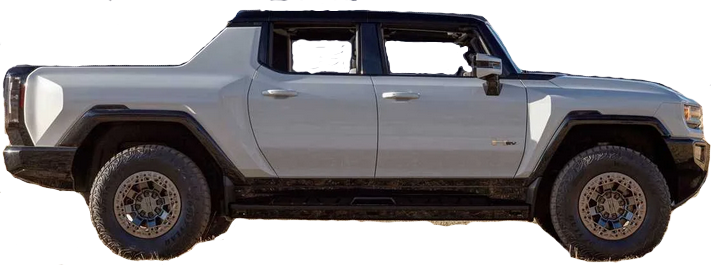
\includegraphics[width=15 mm]{hummer-ev.png} \else \tikz \draw[fill, black] (0,0) rectangle (1,1); \fi};
            \draw[->, black!90, semithick] (-1, 0.16) -- (9 , 0.16) node[below, pos=1] {$X$};
        \end{tikzpicture}
      }
    \end{animateinline}
  \end{center}
}

\begin{document}

\maketitle


\begin{frame}[label=A1]{Un sistema mecánico}

  
  \hummeranimation{1}

  \alert{Actividad} Identifica y indica con flechas todas las fuerzas que afectan el coche. Para cada fuerza identifica y indica su contra-fuerza.

\end{frame}


\note{%
}

\begin{frame}[label=I1]{Intuición para sistemas mecánicos}

  Un coche va a velocidad constante en una autopista horizontal. En el instante $t=t_1$, el conductor pone la transmisión en 'N', desconectando el motor de las ruedas. Cuál de las siguientes graficas describe mejor la velocidad $v(t)=\dot{X}(t)$ del coche?

  \begin{center}
    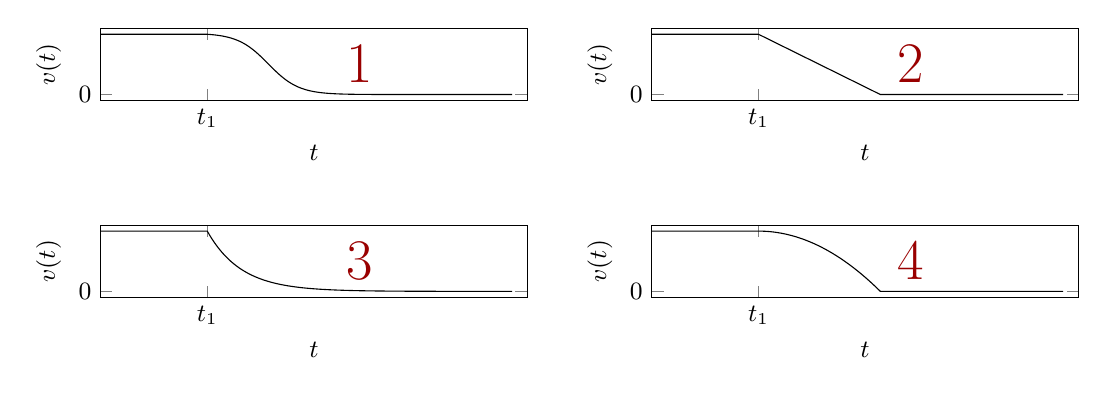
\begin{tikzpicture}
      \small

      \begin{axis}[
        width=7cm,
        height=2.5cm,
        xlabel={$t$},
        ylabel={$v(t)$},
        xmin=-3.5,
        xmax=10.5,
        ytick = {0},
        xtick = {0},
        xticklabels = {$t_1$},
        ]
        \addplot+[black, no marks, domain=-4:10, samples=400,variable=k] { (k < 0) + (k>0)*(1+exp(-4))/(1+exp(4*(0.5*k-1)))};

        \node[black!40!red] at (axis cs: 5, 0.5) {\huge 1};
      \end{axis}

      \begin{axis}[
        xshift=7cm,
        width=7cm,
        height=2.5cm,
        xlabel={$t$},
        ylabel={$v(t)$},
        xmin=-3.5,
        xmax=10.5,
        ytick = {0},
        xtick = {0},
        xticklabels = {$t_1$},
        ]
        \addplot+[black, no marks, domain=-4:10, samples=400,variable=k] { (k<0) + ((k>=0) - (k>4))*(1/4*(4-k)) };
        \node[black!40!red] at (axis cs: 5, 0.5) {\huge 2};
      \end{axis}

      \begin{axis}[
        xshift=0cm,
        yshift=-2.5cm,
        width=7cm,
        height=2.5cm,
        xlabel={$t$},
        ylabel={$v(t)$},
        xmin=-3.5,
        xmax=10.5,
        ytick = {0},
        xtick = {0},
        xticklabels = {$t_1$},
        ]
        \addplot+[black, no marks, domain=-4:10, samples=400,variable=k] { (k<0) + (k>0)*exp(-0.9*k)};
        \node[black!40!red] at (axis cs: 5, 0.5) {\huge 3};
      \end{axis}

      \begin{axis}[
        xshift=7cm,
        yshift=-2.5cm,
        width=7cm,
        height=2.5cm,
        xlabel={$t$},
        ylabel={$v(t)$},
        xmin=-3.5,
        xmax=10.5,
        ytick = {0},
        xtick = {0},
        xticklabels = {$t_1$},
        ]
        \addplot+[black, no marks, domain=-4:10, samples=400,variable=k] { (k<0) + ((k>=0) - (k>4))*(1-1/16*pow(-k,2)) };
        \node[black!40!red] at (axis cs: 5, 0.5) {\huge 4};
      \end{axis}


    \end{tikzpicture}

  \end{center}

\end{frame}

\begin{frame}[label=M1]{Modelación}

  \hummeranimation{1}

  \begin{center}
    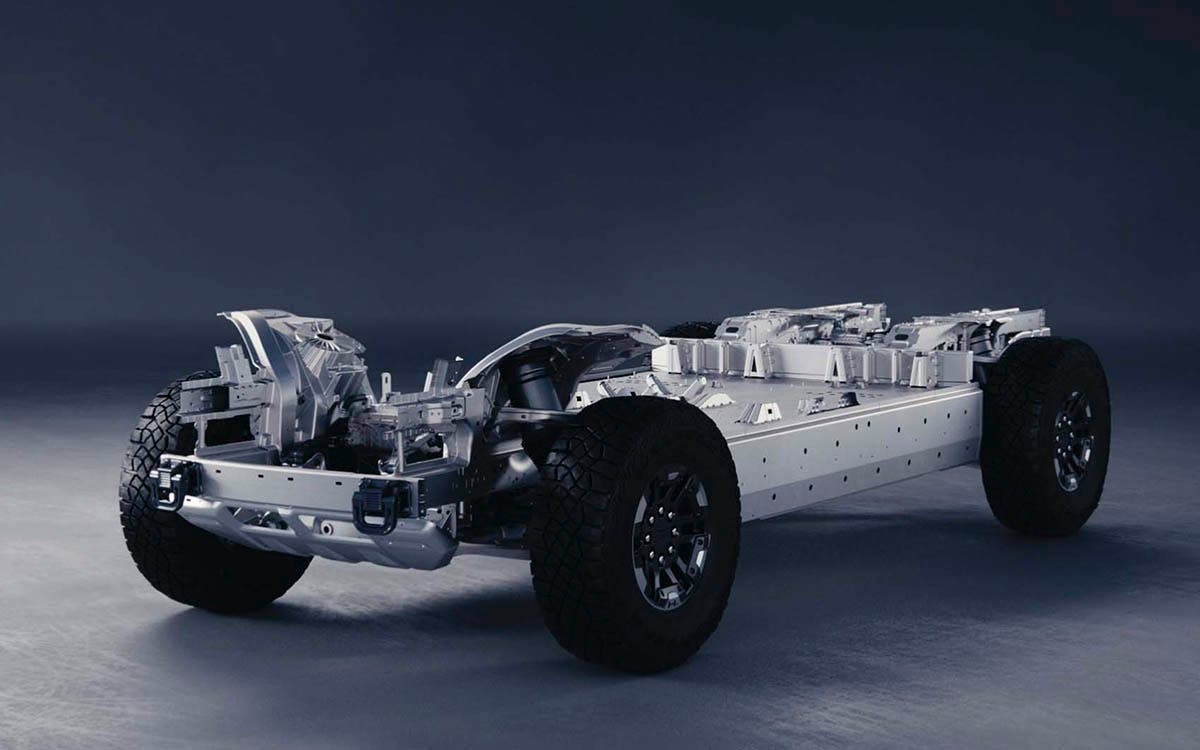
\includegraphics[height=4cm]{hummer-ev.jpg}
  \end{center}
  ¿Cómo \alert{modelar} este sistema?  Depende del \alert{propósito}: ¿Para qué necesitamos el modelo?
\end{frame}

\begin{frame}[label=M2]{Simplificar}

  \hummeranimation{0} % Just black box

  \begin{center}
    \begin{tikzpicture}
      \node[] (hev) {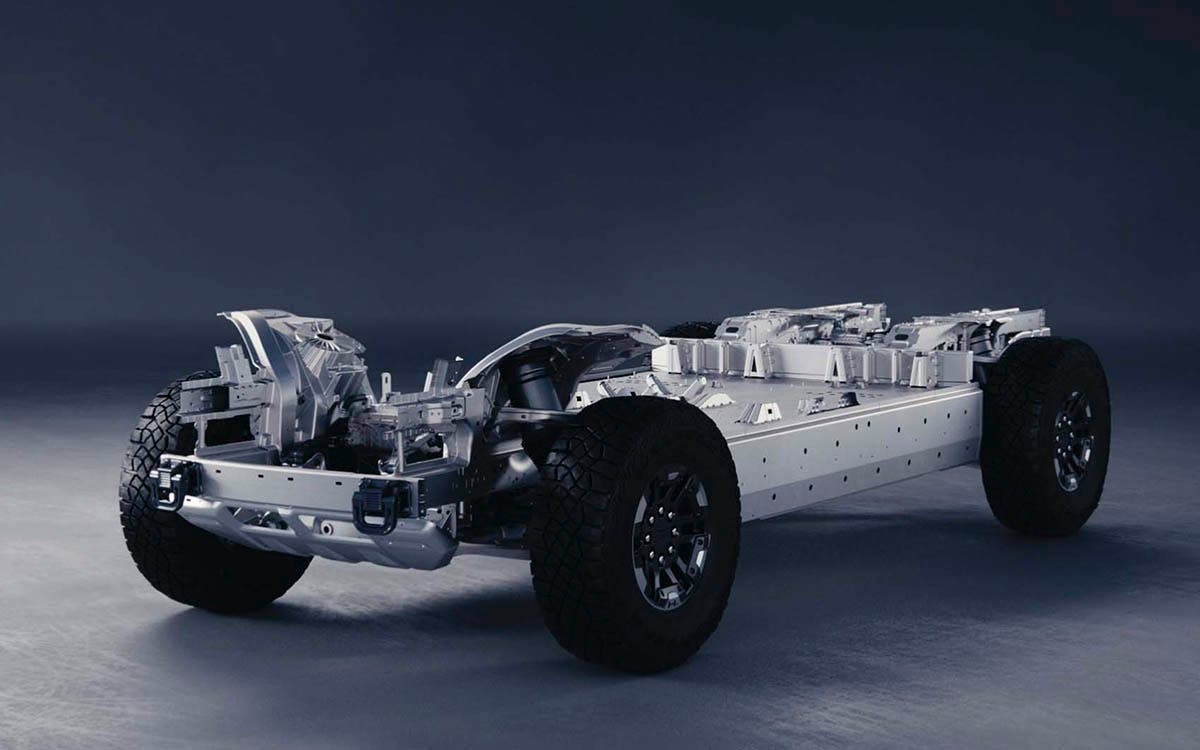
\includegraphics[height=2cm]{hummer-ev.jpg}};
      \node[draw, fill, right of=hev, node distance=2 cm, minimum height=0.3cm, minimum width=0.3cm] (pm) {};

      \draw[thick, ->] (hev) to (pm);
    \end{tikzpicture}
  \end{center}
\end{frame}

\begin{frame}[label=M3]{Modelo de masa puntual}

  La segunda ley de Newton: ``Masa por acceleración es igual a la suma de las fuerzas''
  \[ \frac{d}{dt} (mv) = \sum_i F_i\]
  \begin{center}
    \small 
    \begin{tikzpicture}[scale=1.4, transform shape]
      \node[anchor=south,] at (1, 0) (hummer) {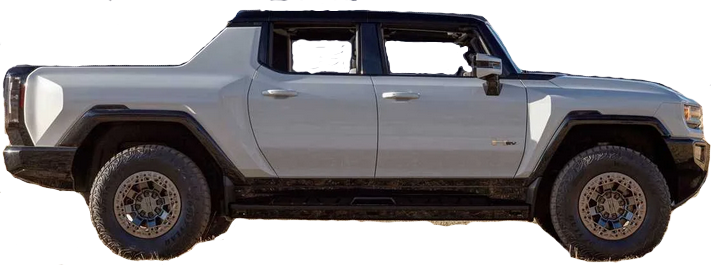
\includegraphics[width=15 mm]{hummer-ev.png}};
      \node[coordinate] (com) at ($ (hummer.center) + (0.15, 0) $) {};
      \node[coordinate] (wheels) at ($ (hummer.south) + (0, 0.16) $) {};
      
      \draw[->, black!90, semithick] (-1, 0.16) -- (9 , 0.16) node[below, pos=1] {$X$};
      \draw[->, black!90, ] (-1, 0.16) -- (-1 , 3) node[left, pos=1] {$Y$};
      
      \draw[thick, green!70!black, ->] (com) -- ++(0, -2cm) node[right] {$F_g = mg$};
      \draw[thick, orange!80!black, ->] (wheels) -- ++(0, 1.3cm) node[right] {$F_{n}$};
      \draw[thick, red!80!black, ->] (wheels) -- ++(2cm, 0) node[below] {$F_m$};
      \draw[thick, blue!80!black, <-] (hummer.east) -- ++(2cm, 0) node[above] {$F_d$};

    \end{tikzpicture}
  \end{center}

  No hay acceleración en la dirección $Y$ (equilibrio en las fuerzas perpendiculares al suelo)
  \[ 0 = F_{n} - F_g \quad \Rightarrow \quad F_{n} = F_g = mg\]
  En la dirección $X$:
  \[ m\dot{v} = F_m - F_d\]
\end{frame}

% Masa puntual?
\begin{frame}[label=M4]{Modelo de masa puntual}
  \[ m\dot{v} = F_m - F_d\]
  Modelo cuadratico del arrastre \(F_d = \sign(v)kv^2\).

\begin{center}
    \begin{tikzpicture}
      \begin{axis}[
        axis lines = middle,
        ytick=\empty,
        xtick=\empty,
        xlabel={$v$},
        ylabel={$F_d$},
        ]
        
        \addplot [blue!80, smooth, domain=-4:4] { sign(x)*x*x};

      \end{axis}
    \end{tikzpicture}
  \end{center}
  \[ m\dot{v} + \sign(v)kv^2 = F_m, \qquad \text{Ecuación diferencial nonlineal}\]
\end{frame}

 \pgfplotstableread[col sep=comma]{car-drag-60.dta}{\cardragtable}

\begin{frame}[label=M5E]{Modelo de masa puntual}

  \[ \dot{v} = \frac{1}{m}(F_m - \sign(v)kv^2)\]

  Inicialmente a $t=0$ el coche está parado, y la fuerza del motor sube de 0 a $F_m$ y se queda constante. Cómo se comporta el sistema?

    \begin{center}
    \begin{tikzpicture}
      \small

      \begin{axis}[
        width=7cm,
        height=2.5cm,
        xlabel={$t$},
        ylabel={$v(t)$},
        xmin=-0.5,
        xmax=6,
        ytick = {0},
        xtick = {0},
        %xticklabels = {$t_1$},
        ]
        \addplot+[black, no marks, domain=-1:6, samples=200, smooth, variable=k] { (k>=0)*(exp(1.6*(k-3))/(1+exp(1.6*(k-3))))};

        \node[black!40!red] at (axis cs: 5, 0.5) {\huge 1};
      \end{axis}

      \begin{axis}[
        xshift=7cm,
        width=7cm,
        height=2.5cm,
        xlabel={$t$},
        ylabel={$v(t)$},
        xmin=-0.5,
        xmax=6,
        ytick = {0},
        xtick = {0},
        %xticklabels = {$t_1$},
        ]
        \addplot+[black, no marks, smooth] table[col sep=comma, y index = 2] {car-drag.dta};
        \node[black!40!red] at (axis cs: 5, 1) {\huge 2};
      \end{axis}

      \begin{axis}[
        xshift=0cm,
        yshift=-2.5cm,
        width=7cm,
        height=2.5cm,
        xlabel={$t$},
        ylabel={$v(t)$},
        xmin=-0.5,
        xmax=6,
        ytick = {0},
        xtick = {0},
        %xticklabels = {0},
        ]
        \addplot+[black, no marks, domain=-4:10, samples=100, smooth, variable=k] { (k>0)*(k<4)*(1/4*k) + (k>4) };
        \node[black!40!red] at (axis cs: 5, 0.5) {\huge 3};
      \end{axis}

      \begin{axis}[
        xshift=7cm,
        yshift=-2.5cm,
        width=7cm,
        height=2.5cm,
        xlabel={$t$},
        ylabel={$v(t)$},
        xmin=-0.5,
        xmax=6,
        ytick = {0},
        xtick = {0},
        %xticklabels = {$t_1$},
        ]
        \addplot+[black, no marks, domain=-4:10, samples=100, smooth, variable=k] { (k>0)*(k<4)*1/16*pow(k,2)) + (k>4) };
        \node[black!40!red] at (axis cs: 5, 0.5) {\huge 4};
      \end{axis}


    \end{tikzpicture}

  \end{center}
\end{frame}

\begin{frame}[label=M6A]{Modelo de masa puntual}
  \[ \dot{v} = \frac{1}{m}(F_m - \sign(v)kv^2) \]
  \begin{center}
    \begin{animateinline}[]{20}
      \multiframe{60}{n=1+1}{
        \pgfplotstablegetelem{\n}{2}\of\cardragtable
        \pgfmathsetmacro{\xpos}{\pgfplotsretval}
        \begin{tikzpicture}
          \begin{axis}[
            axis lines = middle,
            ytick={4},
            yticklabels={$\frac{F_m}{m}$},
            xtick=\empty,
            xlabel={$v$},
            ylabel={$\dot{v}$},
            ymax=5,
            clip=false,
            ]
            \addplot [orange!80, smooth, domain=0:2.4] {4-sign(x)*x*x};
            \draw[blue!70, fill] (axis cs: \xpos, 0) circle[radius=5pt];
      \end{axis}
    \end{tikzpicture}
}
\end{animateinline}
\end{center}
\end{frame}

\begin{frame}[label=L1]{Modelo del arrastre}

  \[ m\dot{v} = F_m - F_d\]
  Modelo del arrastre incluyendo resistencia a la rodadura \(F_d = \sign(v)(r + kv^2)\).
  \[ m\dot{v} = F_m -\sign(v)(r + kv^2)\]
  
\begin{center}
    \begin{tikzpicture}[scale=0.7
      \begin{axis}[
        axis lines = middle,
        ytick=\empty,
        xtick=\empty,
        xlabel={$v$},
        ylabel={$F_d$},
        ]
        
        \addplot [blue!80, domain=-4:4, samples=800] { sign(x)*(0.4 + x*x)};

      \end{axis}
    \end{tikzpicture}
  \end{center}
  Problema: El diseño de un controlador de velocidad necesita un modelo \alert{lineal}. El modelo arriba es \alert{nonlineal}.

\end{frame}

\begin{frame}[label=L2A]{Linealización}
  \begin{columns}
    \begin{column}{0.4\columnwidth}
      \begin{align*}
        f(v) &= \sign(v)(r + kv^2) \\&= \begin{cases} r + kv^2, & v\ge 0\\-r-kv^2, & v<0 \end{cases}\\
             &\approx f(v_0) + \frac{df}{dv}\big|_{v_0}(v - v_0)\\
        \frac{df}{dv} &= \begin{cases} 2kv, & v>0\\-2kv, & v<0\\\text{indefinido}, & v=0 \end{cases}
      \end{align*}
    \end{column}

    \begin{column}{0.6\columnwidth}
    \begin{center}
    \begin{animateinline}[controls, palindrome]{2}
      \multiframe{16}{n=-3.2+0.44}{
        \begin{tikzpicture}[scale=0.8]
        \pgfmathsetmacro{\vnull}{\n}
          \begin{axis}[
            axis lines = middle,
            ytick=\empty,
            xtick={\vnull},
            xticklabels={$v_0$},
            xlabel={$v$},
            ylabel={$F_d$},
            clip=false,
            xmin=-6,
            xmax=6,
            ymin=-20,
            ymax=20,
            ]
           
            \addplot [blue!80, domain=-4:4, samples=400, thick] { sign(x)*(0.4 + x*x)};
            %\addplot [orange!80, domain=-1.5:1.5, samples=4, variable=\t] ({t}, {t});
            \addplot [orange!80, domain=-1.5:1.5, samples=4, variable=\t, thick] ({t+\vnull}, {sign(\vnull)*(0.4 + pow(\vnull, 2)) + (2*abs(\vnull))*t} );
          \end{axis}
        \end{tikzpicture}
      }
    \end{animateinline}
  \end{center}
\end{column} 
\end{columns}
\end{frame}

\end{document}
